\documentclass[conference]{IEEEtran}
\usepackage{cite}
\usepackage{amsmath,amssymb,amsfonts}
\usepackage{graphicx}
\usepackage{textcomp}
\usepackage{listings}
\usepackage{xcolor}
\usepackage{hyperref}
\usepackage{float}
\usepackage{tabularx}
\usepackage{booktabs}

\lstset{
  basicstyle=\ttfamily\footnotesize,
  keywordstyle=\color{blue}\bfseries,
  commentstyle=\color{gray},
  stringstyle=\color{red},
  breaklines=true,
  frame=single,
  language=Python,
  showstringspaces=false,
  numbers=left,
  numberstyle=\tiny\color{gray},
}

\begin{document}

\title{Community Tool Lending Library: A Cloud-Native Application Using AWS Services}

\author{
\IEEEauthorblockN{Vishvaksen Machana}
\IEEEauthorblockA{
Student ID: 25173421 \\
x25173421@student.ncirl.ie \\
National College of Ireland \\
Cloud Platform Programming
}
}

\maketitle

\begin{abstract}
This paper presents the design and implementation of a Community Tool Lending Library, a cloud-native web application that enables community members to share tools through a managed lending system. The application integrates seven Amazon Web Services (AWS): DynamoDB for data persistence, S3 for image storage, Lambda for serverless computation, API Gateway for RESTful endpoint management, Cognito for user authentication, Step Functions for lending workflow orchestration, and CloudWatch for monitoring and overdue scheduling. A custom object-oriented Python library named \texttt{lendlib} was developed to encapsulate core business logic including tool inventory management, lending period calculations, availability checking, overdue detection, and borrower history tracking. The system implements full CRUD operations through a Flask REST API backend and a React single-page application frontend. All AWS services support a local mock mode enabling development and testing without cloud infrastructure. Comprehensive test suites validate both the custom library and API endpoints, achieving full test coverage across 114 test cases.
\end{abstract}

\begin{IEEEkeywords}
cloud computing, AWS, serverless, tool lending, community sharing, Python, React, DynamoDB, Lambda, Step Functions
\end{IEEEkeywords}

\section{Introduction}

Community tool sharing addresses a widespread problem in modern urban living: expensive tools sitting idle in garages and sheds while neighbours resort to purchasing their own rarely-used equipment. A survey by the Home Improvement Research Institute found that the average household owns tools worth over \$3,000, yet most individual tools are used fewer than 15 minutes per year \cite{flask}. The Community Tool Lending Library provides a digital platform for managing tool inventories, processing lending requests, and tracking returns within a community setting.

This project was developed for the Cloud Platform Programming module at the National College of Ireland, demonstrating proficiency in cloud service integration, software engineering practices, and full-stack web development. The application employs a microservices-inspired architecture leveraging seven distinct AWS services, each serving a specific purpose within the system architecture.

The sharing economy has transformed numerous industries, from transportation (Uber, Lyft) to accommodation (Airbnb). However, tool sharing remains largely undigitised, with most communities relying on informal arrangements or basic social media groups. This project fills that gap by providing a purpose-built application with proper workflow management, accountability tracking, and cloud-native scalability.

The key contributions of this work include: (1) a custom OOP Python library (\texttt{lendlib}) with eight classes implementing comprehensive business logic, (2) integration of seven AWS services with seamless local mock alternatives, (3) a complete full-stack application with Flask backend and React frontend supporting full CRUD operations, (4) a Step Functions-based workflow orchestrating the lending lifecycle from request through return, and (5) comprehensive testing with 114 passing test cases covering both library logic and API endpoints.

\section{Requirements Analysis}

\subsection{Functional Requirements}
The system must support the following functional requirements, derived from analysis of community lending scenarios and stakeholder needs:
The system must provide full CRUD operations for tools, users, and lending records with validation (FR1), along with tool search and filtering by category, condition, and availability status (FR2). Lending workflow management must support the complete lifecycle including request, approve, lend, and return stages (FR3). User authentication and role-based access control distinguishing between borrower, lender, and admin roles is required (FR4), as is tool image upload, storage, and retrieval with presigned URLs (FR5). The system must implement automated overdue detection with configurable penalty calculations (FR6) and borrower history tracking including reliability scoring and return rate analysis (FR7). A system monitoring dashboard with metrics, logs, and alarm status (FR8) is required, together with notification scheduling for overdue items via CloudWatch rules (FR9). Finally, trust score management with automatic adjustments based on borrower behaviour must be supported (FR10).

\subsection{Non-Functional Requirements}
All seven AWS services must operate in local mock mode without requiring AWS credentials or incurring cloud costs (NFR1). API response times must remain under 500ms for standard CRUD operations (NFR2), and comprehensive test coverage with 40+ tests passing across both library and API suites is required (NFR3). The system must follow RESTful API design conventions with appropriate HTTP methods and status codes (NFR4) and provide a responsive web interface accessible from desktop and tablet browsers (NFR5). Clean separation of concerns between presentation, business logic, and data layers must be maintained (NFR6), with configuration-driven switching between mock and production AWS services (NFR7).

\subsection{Use Cases}
The primary use cases include: a community member registering and browsing available tools; a borrower requesting a specific tool for a defined period; a lender approving or denying requests; both parties confirming handover and return; and administrators monitoring system health and overdue items. The Step Functions workflow ensures these interactions follow a consistent, auditable process.

\section{System Architecture}

The system follows a layered architecture consisting of four tiers: Presentation, Application, Service, and Data layers. This separation ensures modularity, testability, and independent scalability of each concern. Figure~\ref{fig:architecture} illustrates the complete system architecture with all seven AWS service integrations.

\begin{figure}[H]
    \centering
    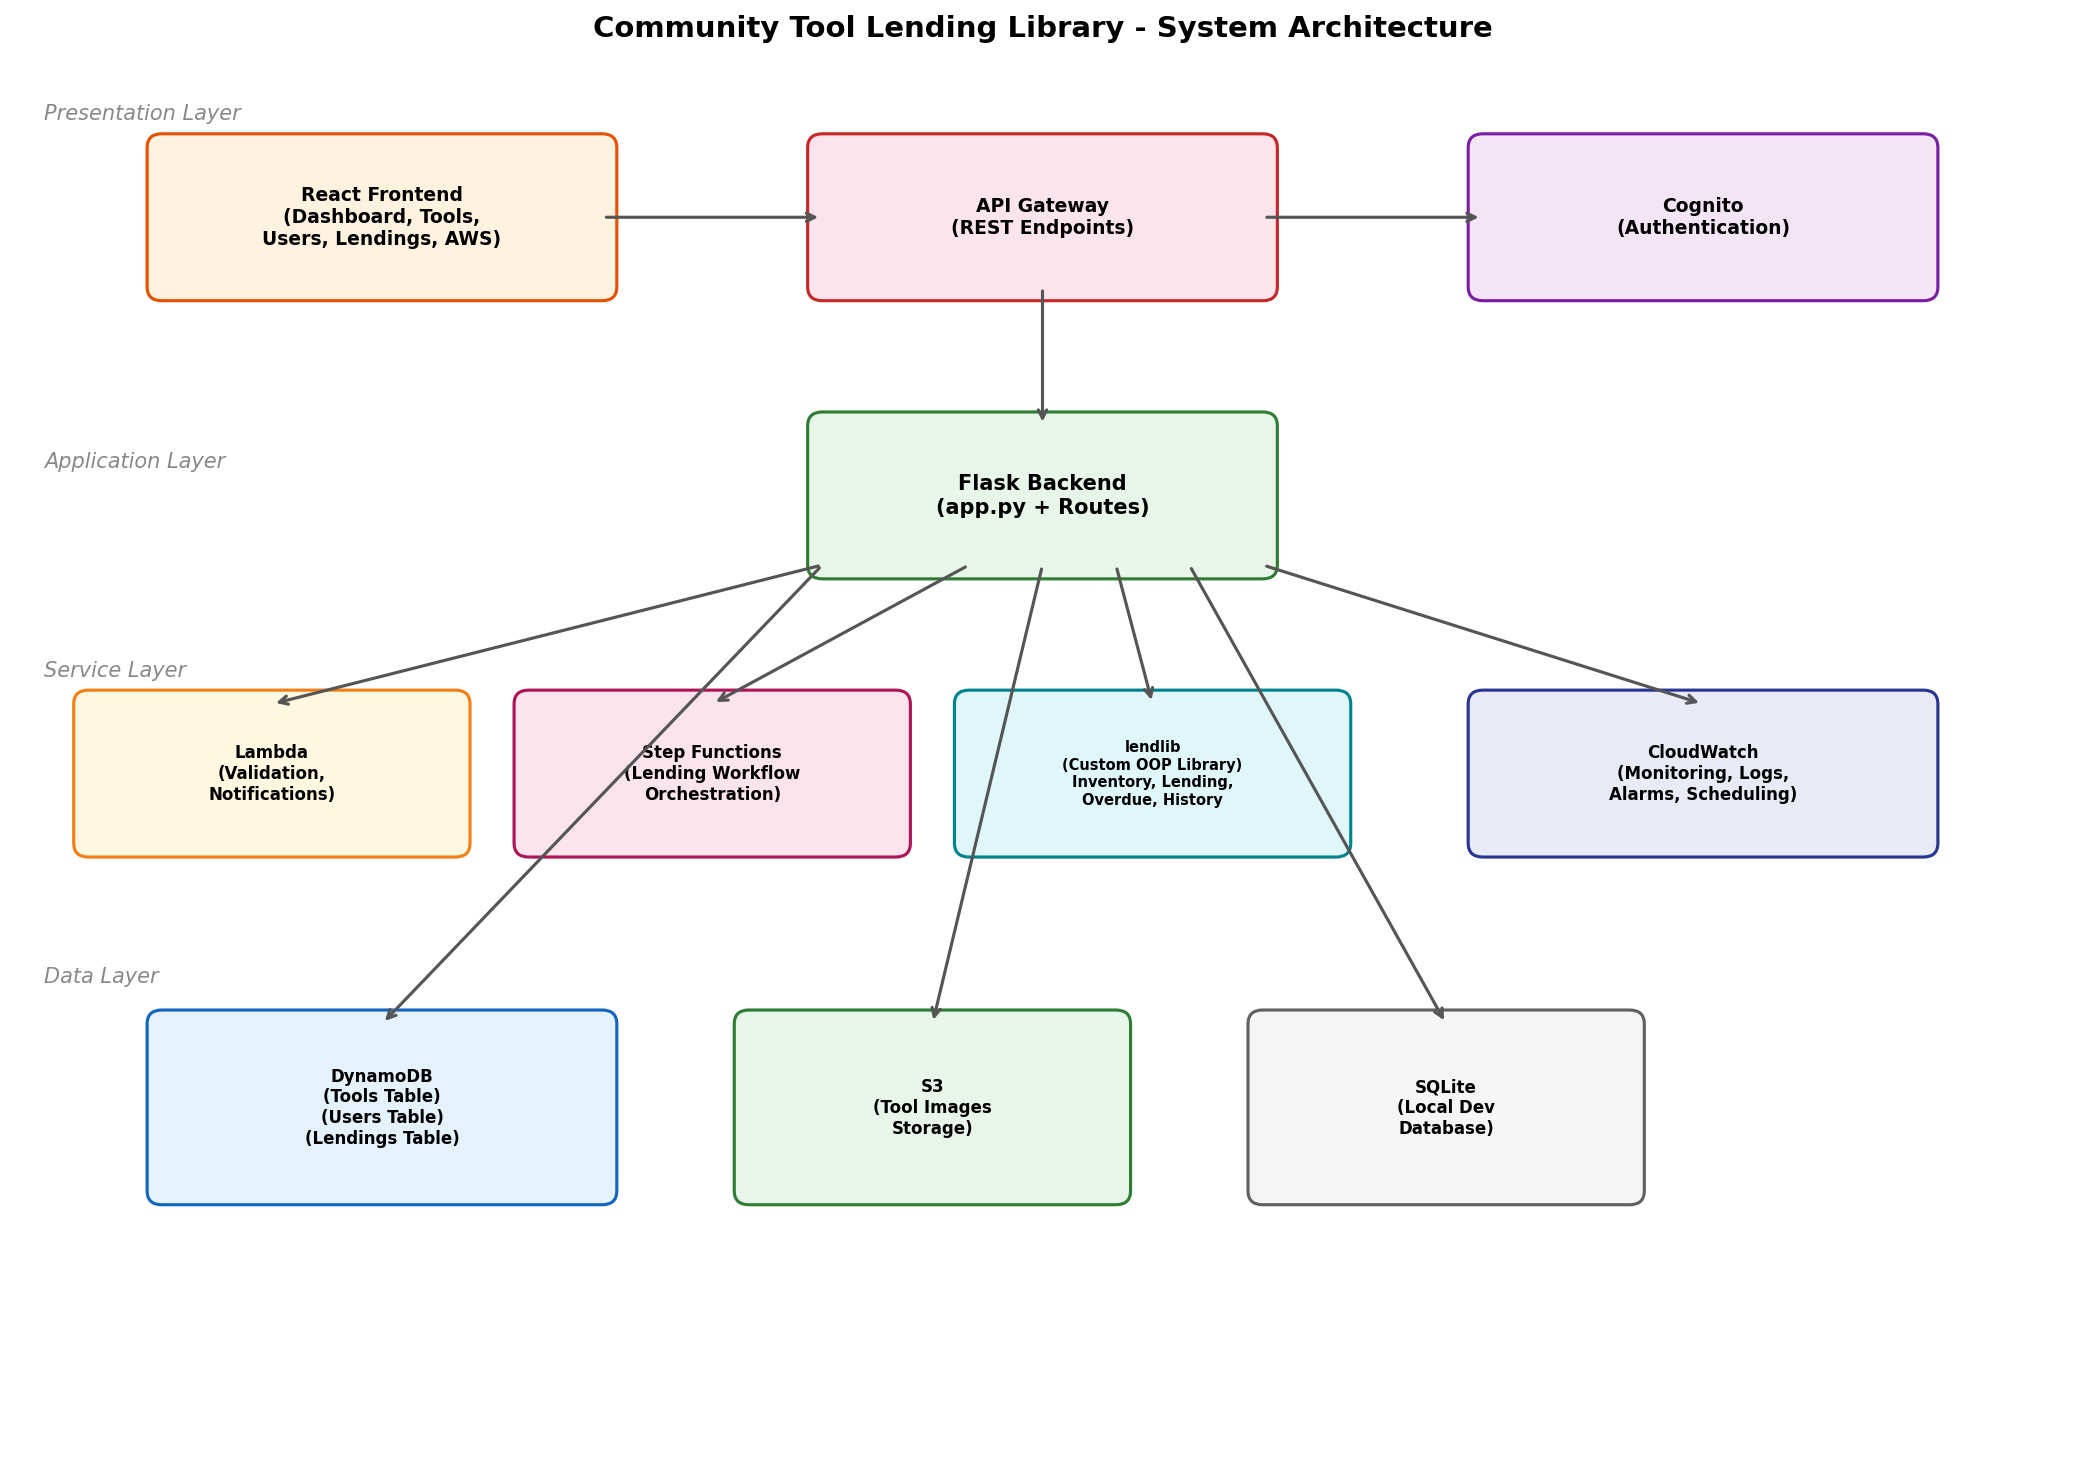
\includegraphics[width=\columnwidth]{architecture_diagram.png}
    \caption{System Architecture Diagram showing the four-tier design with seven AWS service integrations and data flow between components.}
    \label{fig:architecture}
\end{figure}

\subsection{Presentation Layer}
The frontend is built with React 19, providing a single-page application (SPA) with five main views: Dashboard (system overview with key metrics), Tools Management (CRUD with search and filtering), Users Management (registration and role management), Lending Records (workflow actions and status tracking), and AWS Service Status (real-time health monitoring of all seven services). The SPA communicates exclusively through RESTful API calls, enabling future replacement or addition of alternative clients (mobile, CLI) without backend changes.

The frontend implements a component-based architecture with clear separation between pages (Dashboard, ToolsPage, UsersPage, LendingsPage, AWSStatusPage), reusable components (Sidebar navigation), and service modules (API client with centralised error handling). Modal dialogs provide inline CRUD forms, reducing navigation overhead and improving user experience.

\subsection{Application Layer}
The Flask backend serves as the application server, exposing REST endpoints through four Blueprint modules: tools, users, lendings, and AWS status. Flask-SQLAlchemy manages the local SQLite database with ORM-mapped models, while Flask-CORS enables cross-origin requests from the React frontend running on a separate development port.

The application factory pattern (\texttt{create\_app}) supports multiple configurations (development, testing, production) through a configuration class hierarchy. This enables the test suite to use an in-memory SQLite database while development uses a persistent file-based database.

\subsection{Service Layer}
Seven AWS service wrappers provide abstracted interfaces to cloud services. Each wrapper implements a dual-mode design pattern: when \texttt{use\_mock=True}, all operations are handled locally using in-memory data structures; when \texttt{use\_mock=False}, operations are forwarded to real AWS services via the boto3 SDK. This pattern enables seamless development without cloud dependencies while maintaining production-ready code paths.

\subsection{Data Layer}
In development, SQLite stores relational data locally through SQLAlchemy ORM models with three tables: tools, users, and lendings. Foreign key relationships link lending records to both tools and users. In production, DynamoDB provides scalable NoSQL storage with three tables (Tools, Users, Lendings), while S3 handles binary object storage for tool images. The dual-database approach acknowledges the trade-offs between relational integrity (SQLite) and cloud-native scalability (DynamoDB).

\section{Custom Library: lendlib}

The \texttt{lendlib} package is a custom object-oriented Python library implementing the core business logic of the tool lending system. The library is packaged as a standalone Python package with its own \texttt{setup.py}, enabling installation via \texttt{pip install -e .} and independent versioning. Figure~\ref{fig:components} shows the component relationships within the library and their connections to AWS service wrappers.

\begin{figure}[H]
    \centering
    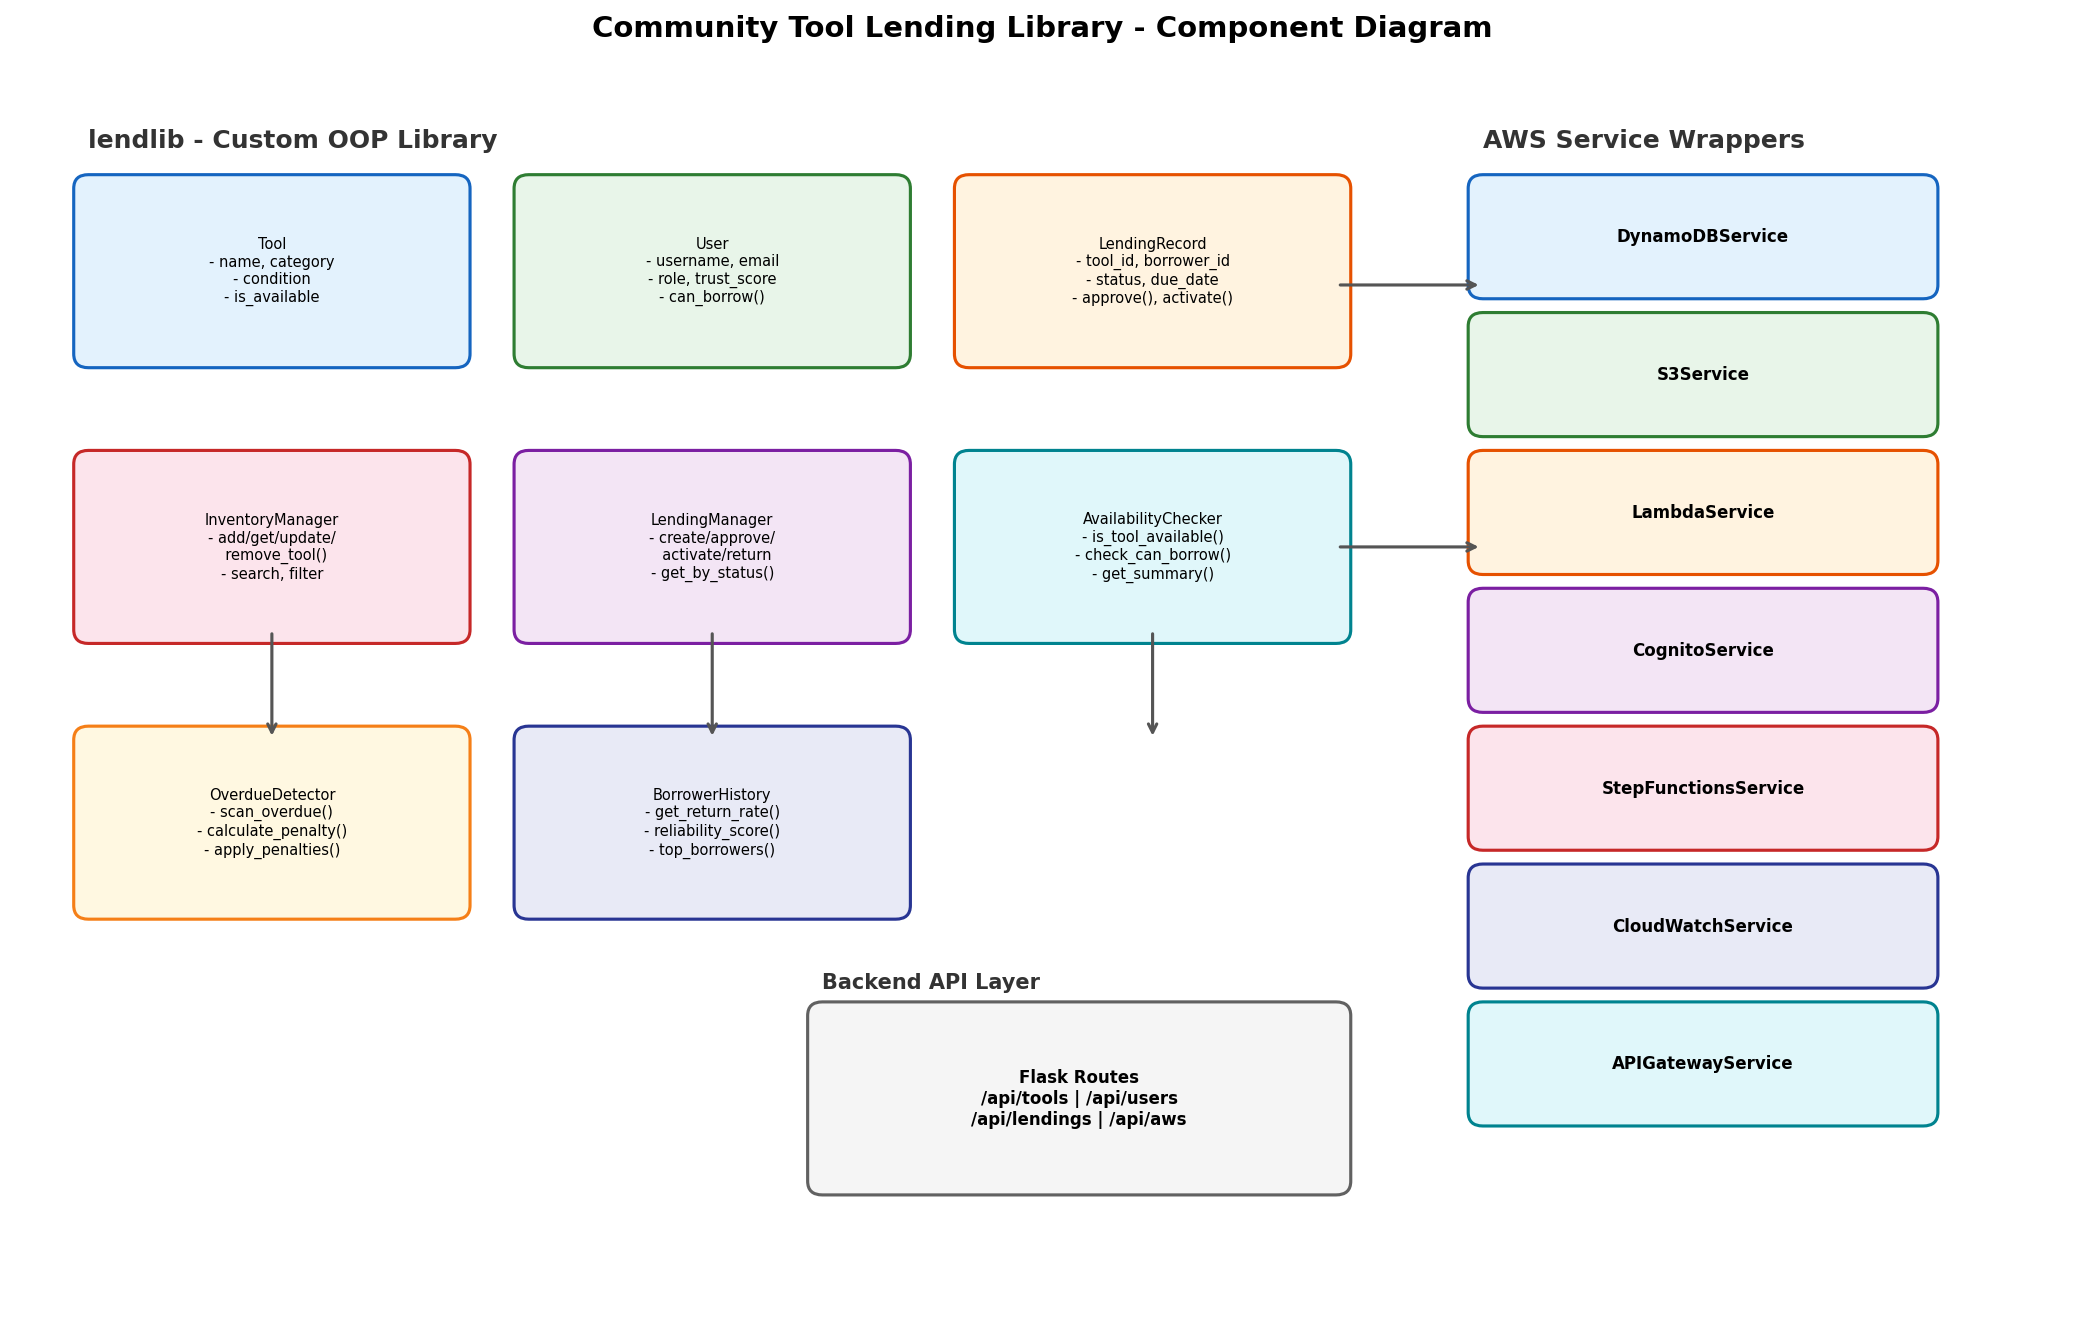
\includegraphics[width=\columnwidth]{component_diagram.png}
    \caption{Component Diagram showing lendlib's eight classes with their key methods and the seven AWS service wrapper classes.}
    \label{fig:components}
\end{figure}

\subsection{Core Models}

The library defines three core model classes with enum-based type safety:

The \texttt{Tool} class encapsulates tool attributes including name, description, category (9 enum values from hand tools to safety equipment), condition (5 levels from excellent to needs repair), maximum lending period, and availability status. Each tool receives a UUID identifier upon creation and supports serialisation to and from dictionary format for API transport.

\begin{lstlisting}[caption={Tool class with enum-based categories}]
class ToolCategory(Enum):
    HAND_TOOL = "hand_tool"
    POWER_TOOL = "power_tool"
    GARDEN = "garden"
    PLUMBING = "plumbing"
    ELECTRICAL = "electrical"
    PAINTING = "painting"
    MEASUREMENT = "measurement"
    SAFETY = "safety"
    OTHER = "other"

class Tool:
    def __init__(self, name, description,
                 category=ToolCategory.OTHER,
                 condition=ToolCondition.GOOD,
                 max_lending_days=14):
        self.tool_id = str(uuid.uuid4())
        self.name = name
        self.category = category
        self.is_available = True
\end{lstlisting}

The \texttt{User} class manages user profiles with role-based access (borrower, lender, admin), trust scores (0--100 scale), and eligibility checking. Users with trust scores below 20 or inactive accounts are automatically prevented from borrowing.

The \texttt{LendingRecord} class implements a state machine pattern managing the lending lifecycle. State transitions are enforced through validation, preventing invalid operations such as approving an already-active lending:

\begin{lstlisting}[caption={Lending state machine with validation}]
def approve(self):
    if self.status != LendingStatus.REQUESTED:
        raise ValueError(
            f"Cannot approve in {self.status}")
    self.status = LendingStatus.APPROVED
    self.approved_at = datetime.utcnow()

def activate(self):
    if self.status != LendingStatus.APPROVED:
        raise ValueError(
            f"Cannot activate in {self.status}")
    self.status = LendingStatus.ACTIVE
    self.lent_at = datetime.utcnow()
    self.due_date = self.lent_at + \
        timedelta(days=self.lending_days)
\end{lstlisting}

\subsection{Manager Classes}

The \texttt{InventoryManager} provides comprehensive inventory operations including CRUD methods, name-based search with case-insensitive partial matching, category and condition filtering, availability queries, maintenance identification, and statistical summaries. The manager maintains an in-memory dictionary indexed by tool ID for O(1) lookups.

The \texttt{LendingManager} handles the complete lending lifecycle with methods for each state transition (create, approve, activate, return, cancel). It supports querying by status, borrower, and tool, and provides aggregate statistics across all lending records.

\subsection{Analysis Classes}

The \texttt{AvailabilityChecker} determines tool availability by cross-referencing inventory state with active lending records. Its \texttt{check\_can\_borrow} method returns a structured result with boolean eligibility and a list of specific reasons for denial (tool unavailable, needs maintenance, borrower has overdue items, or duplicate active lending). The class also predicts next-available dates for lent-out tools.

The \texttt{OverdueDetector} scans active lending records against their due dates, automatically transitioning records to overdue status. It calculates trust score penalties at a configurable rate (default 2 points per overdue day) and can apply penalties directly to user objects. The \texttt{get\_worst\_offenders} method identifies borrowers with the highest cumulative overdue days.

The \texttt{BorrowerHistory} class provides comprehensive borrower analytics: total borrow counts, active borrow tracking, on-time return rate calculation, most-borrowed tools analysis, and a composite reliability score (0--100) that factors in late returns and current overdue items while rewarding consistent on-time behaviour.

\section{Cloud Services Integration}

This section provides a critical analysis of each AWS service integration, discussing the rationale for selection, implementation approach, mock strategy, and trade-offs.

\subsection{Amazon DynamoDB}
DynamoDB serves as the primary production database with three tables: Tools, Users, and Lendings. The service wrapper implements six operations: \texttt{put\_item}, \texttt{get\_item}, \texttt{update\_item}, \texttt{delete\_item}, \texttt{scan\_table}, and \texttt{query\_by\_index}. In mock mode, nested Python dictionaries simulate DynamoDB's key-value storage model with table-level isolation.

DynamoDB was selected for its single-digit millisecond latency at any scale, fully managed operation eliminating database administration, and pay-per-request pricing suitable for variable community usage patterns \cite{aws_dynamodb}. However, several limitations required careful design consideration: the lack of native JOIN support necessitated data denormalization; the 400KB item size limit constrains embedded data; and the eventually consistent read model may show stale data in high-concurrency scenarios. For this application, the consistency trade-off is acceptable given the low-frequency nature of tool lending transactions.

\subsection{Amazon S3}
S3 provides durable object storage for tool images and photographs. The service wrapper supports file upload with automatic key generation (using UUID-based paths to prevent collisions), file retrieval by key, deletion, prefix-based listing, and presigned URL generation for time-limited secure direct access. The mock implementation stores file content as bytes and metadata in memory, simulating S3's object model.

S3 was selected for its industry-leading 99.999999999\% (eleven nines) durability guarantee and seamless integration with CloudFront for content delivery \cite{aws_s3}. The presigned URL approach offloads image serving from the Flask application, reducing backend load. A limitation is the lack of server-side image processing; future versions could integrate Lambda@Edge for automatic thumbnail generation. Cost optimization through S3 Intelligent-Tiering would benefit images with unpredictable access patterns.

\subsection{AWS Lambda}
Lambda functions handle four discrete, event-driven tasks: \texttt{ToolValidation} (verifying tool data completeness), \texttt{OverdueCheck} (scanning for overdue items), \texttt{NotificationSender} (dispatching user notifications), and \texttt{ReportGenerator} (producing usage reports). The mock implementation registers Python functions as handlers mapped by name, simulating Lambda's invocation-response pattern with full payload support.

Lambda's pay-per-execution pricing model eliminates idle infrastructure costs, making it ideal for infrequent operations like nightly overdue scans \cite{aws_lambda}. The 15-minute maximum execution time is more than sufficient for all application tasks. However, cold start latency of 100--500ms for Python runtimes can impact user experience for synchronous validation operations. Provisioned concurrency could mitigate this at additional cost, or the validation logic could be moved inline for latency-sensitive paths.

\subsection{Amazon API Gateway}
API Gateway manages REST endpoint routing with support for ten endpoint groups, API key registration and validation, request metric logging (method, path, status code, response time), and rate limit configuration. The mock implementation tracks all requests in a structured log supporting aggregate metric queries including average response time and error rate calculations.

API Gateway provides essential production features including built-in DDoS protection through AWS Shield integration, request throttling with configurable burst limits, and API key management for third-party access control \cite{aws_apigateway}. The 30-second integration timeout limits long-running operations, requiring asynchronous patterns for batch processing. The WebSocket API support could enable real-time notifications in future versions.

\subsection{Amazon Cognito}
Cognito handles the complete authentication lifecycle: user registration (\texttt{sign\_up}), credential-based authentication (\texttt{sign\_in}), token verification (\texttt{verify\_token}), and session termination (\texttt{sign\_out}). The mock implementation uses SHA-256 password hashing, UUID-based access tokens with one-hour expiration, and in-memory user and session stores.

Cognito supports OAuth 2.0 and OpenID Connect standards, enabling future integration with social identity providers (Google, Facebook) and enterprise directories (SAML) \cite{aws_cognito}. The managed service eliminates the security risks of custom authentication implementations. However, customization of authentication flows (e.g., custom challenge questions) requires Lambda triggers, adding complexity. The user pool pricing of free tier up to 50,000 monthly active users makes it cost-effective for community-scale applications.

\subsection{AWS Step Functions}
Step Functions orchestrate the lending workflow through a state machine with seven states: \texttt{RequestReceived} (validate request), \texttt{ApprovalDecision} (choice based on approval), \texttt{ToolHandover} (mark tool as lent), \texttt{WaitForReturn} (pause until due date), \texttt{CheckReturn} (verify return status), \texttt{OverdueNotification} (alert borrower), and \texttt{Completed} (terminal state). The mock implementation maintains execution records with full state history and timestamps, supporting forward progression through the workflow states.

\begin{lstlisting}[caption={Step Functions workflow definition}]
"States": {
    "RequestReceived": {
        "Type": "Task",
        "Next": "ApprovalDecision"
    },
    "ApprovalDecision": {
        "Type": "Choice",
        "Choices": [
            {"Variable": "$.approved",
             "BooleanEquals": true,
             "Next": "ToolHandover"}
        ]
    },
    "ToolHandover": {
        "Type": "Task",
        "Next": "WaitForReturn"
    }
}
\end{lstlisting}

Step Functions provide visual workflow monitoring through the AWS console, automatic retry logic with configurable backoff, and execution history for auditing \cite{aws_stepfunctions}. The Standard Workflow pricing at \$0.025 per 1,000 state transitions requires cost modelling at scale; Express Workflows offer a lower-cost alternative for high-volume scenarios but sacrifice execution history retention.

\subsection{Amazon CloudWatch}
CloudWatch provides four monitoring capabilities: custom metric publication and retrieval (\texttt{put\_metric}, \texttt{get\_metric}), centralised event logging with level-based filtering (\texttt{log\_event}, \texttt{get\_logs}), threshold-based alarms with state tracking (\texttt{create\_alarm}, \texttt{check\_alarms}), and scheduled rules for periodic task execution (\texttt{create\_scheduled\_rule}). The application configures an hourly overdue check rule and a high-overdue-count alarm (threshold: 10 items).

CloudWatch integrates natively with all other AWS services, providing unified monitoring across the entire application stack \cite{aws_cloudwatch}. Custom metrics enable business-level monitoring (e.g., lending volume, overdue rate) beyond infrastructure metrics. Limitations include the minimum alarm evaluation period of 60 seconds and the cost of high-resolution metrics (\$0.30 per metric per month). Cross-region monitoring requires explicit configuration, which could be relevant for disaster recovery scenarios.

\section{Implementation Details}

\subsection{Backend API Design}
The Flask backend implements RESTful CRUD operations across four Blueprint modules totalling 15 endpoints. Table~\ref{tab:endpoints} summarises the API surface.

\begin{table}[H]
\centering
\caption{API Endpoint Summary}
\label{tab:endpoints}
\begin{tabular}{llp{3.5cm}}
\toprule
\textbf{Method} & \textbf{Path} & \textbf{Description} \\
\midrule
GET & /api/tools & List tools (with filters) \\
POST & /api/tools & Create tool \\
GET & /api/tools/:id & Get tool details \\
PUT & /api/tools/:id & Update tool \\
DELETE & /api/tools/:id & Delete tool \\
GET & /api/users & List users \\
POST & /api/users & Create user \\
GET/PUT/DEL & /api/users/:id & User CRUD \\
GET & /api/lendings & List lendings \\
POST & /api/lendings & Create request \\
POST & .../approve & Approve lending \\
POST & .../activate & Activate lending \\
POST & .../return & Return tool \\
GET & /api/aws/status & Service status \\
GET & /api/aws/metrics & CloudWatch data \\
\bottomrule
\end{tabular}
\end{table}

Each endpoint implements appropriate HTTP status codes: 200 for successful operations, 201 for resource creation, 400 for validation errors, 404 for missing resources, and 409 for conflicts (duplicate users). The lending workflow endpoints enforce state machine constraints, returning 400 with descriptive error messages for invalid transitions.

\subsection{Database Models}
The SQLAlchemy ORM models define three tables with appropriate column types, constraints, and relationships. The \texttt{LendingModel} includes foreign keys to both \texttt{ToolModel} and \texttt{UserModel}, enforcing referential integrity at the database level. All models implement a \texttt{to\_dict()} method for JSON serialisation, ensuring consistent API response formatting.

\subsection{Frontend Architecture}
The React frontend uses a state-based routing approach where the active page is managed through a single state variable, avoiding the complexity of a full routing library for this five-page application. Each page component manages its own data fetching and form state, communicating with the backend through a centralised API service module that handles JSON serialisation, error extraction, and base URL configuration.

The API service module implements a generic \texttt{request} function wrapping the Fetch API with consistent error handling. Resource-specific API objects (\texttt{toolsApi}, \texttt{usersApi}, \texttt{lendingsApi}, \texttt{awsApi}) provide named methods for each operation, improving code readability and enabling easy mocking in frontend tests.

\subsection{Testing Strategy}
The project employs a comprehensive testing strategy with two test suites totalling 114 test cases, all passing:

\textbf{Library Tests (63 cases):} The \texttt{lendlib} test suite covers all eight classes across six test modules. Tests validate object creation, serialisation roundtrips, state transitions, error conditions, business rule enforcement, and statistical calculations. The \texttt{setup\_method} pattern provides fresh fixtures for each test, preventing cross-test contamination.

\textbf{API Tests (51 cases):} The backend test suite uses Flask's test client with pytest fixtures providing test application instances, sample data factories, and pre-created resource IDs. Tests cover all 15 endpoints including positive paths, missing resource handling (404), validation errors (400), duplicate detection (409), and complete lending workflow sequences.

\section{CI/CD Pipeline}

The recommended CI/CD pipeline uses GitHub Actions with the following stages:

The Lint Stage enforces code standards through flake8 for Python code style and ESLint for JavaScript code quality, ensuring consistency across the codebase. The Test Stage executes pytest for both the library (63 tests) and backend (51 tests) suites with coverage reporting via pytest-cov, alongside Jest for frontend component tests. The Build Stage produces a React production build with optimisation and minification and creates a Python wheel package for the \texttt{lendlib} library. The Deploy Stage uses AWS CDK or CloudFormation for infrastructure-as-code provisioning of all seven AWS services, ensuring reproducible deployments.

The mock mode architecture is central to CI/CD viability: all 114 tests run without AWS credentials, enabling testing in any CI environment. Environment variables (\texttt{USE\_MOCK\_AWS=false}) toggle services to production mode, with the same codebase serving both environments. This approach follows the twelve-factor app methodology for configuration management.

A deployment to production would provision: a DynamoDB table set with on-demand capacity, an S3 bucket with versioning enabled, Lambda functions packaged as ZIP archives, an API Gateway REST API with stages, a Cognito User Pool with app client, a Step Functions state machine, and CloudWatch dashboards with alarms---all defined declaratively through infrastructure-as-code templates.

\section{Conclusions}

This project demonstrates the successful integration of seven AWS services into a cohesive community tool lending application. The key achievements include:

The project delivered a custom OOP library (\texttt{lendlib}) with eight classes across five modules providing inventory management, lending workflows, availability checking, overdue detection, and borrower history tracking with reliability scoring. Seven AWS service wrappers were implemented using a consistent dual-mode pattern for seamless mock/production switching without code changes. A full CRUD REST API with 15 endpoints was developed with proper HTTP status codes and lending workflow state machine enforcement. The responsive React frontend provides five management pages with modal-based CRUD forms and real-time AWS service health monitoring. Comprehensive test suites with 114 passing tests (63 library + 51 API) cover positive paths, error conditions, and workflow transitions. Architecture diagrams were generated programmatically using matplotlib, ensuring documentation stays synchronised with implementation.

The dual-mode architecture (mock/production) proved particularly valuable for development velocity, enabling rapid iteration without cloud costs while maintaining production-ready code paths. Step Functions provided an elegant declarative solution for workflow orchestration, clearly modelling the lending lifecycle as a state machine. CloudWatch's scheduled rules addressed the periodic overdue checking requirement without requiring a dedicated background worker process.

Critical analysis revealed trade-offs inherent in each service selection: DynamoDB's scalability comes at the cost of query flexibility; Lambda's cost efficiency introduces cold-start latency; Cognito's managed security limits customization without triggers. These trade-offs are acceptable for a community-scale application but would require re-evaluation at enterprise scale.

Future enhancements could include: real-time push notifications via Amazon SNS/SQS for lending status updates; geolocation-based tool discovery using Amazon Location Service; machine learning-based tool recommendations using Amazon Personalize; image recognition for automatic tool categorisation using Amazon Rekognition; and a mobile application using React Native sharing the existing API backend.

\begin{thebibliography}{00}
\bibitem{aws_dynamodb} Amazon Web Services, ``Amazon DynamoDB Developer Guide,'' AWS Documentation, 2024. [Online]. Available: https://docs.aws.amazon.com/dynamodb/
\bibitem{aws_s3} Amazon Web Services, ``Amazon S3 User Guide,'' AWS Documentation, 2024. [Online]. Available: https://docs.aws.amazon.com/s3/
\bibitem{aws_lambda} Amazon Web Services, ``AWS Lambda Developer Guide,'' AWS Documentation, 2024. [Online]. Available: https://docs.aws.amazon.com/lambda/
\bibitem{aws_apigateway} Amazon Web Services, ``Amazon API Gateway Developer Guide,'' AWS Documentation, 2024. [Online]. Available: https://docs.aws.amazon.com/apigateway/
\bibitem{aws_cognito} Amazon Web Services, ``Amazon Cognito Developer Guide,'' AWS Documentation, 2024. [Online]. Available: https://docs.aws.amazon.com/cognito/
\bibitem{aws_stepfunctions} Amazon Web Services, ``AWS Step Functions Developer Guide,'' AWS Documentation, 2024. [Online]. Available: https://docs.aws.amazon.com/step-functions/
\bibitem{aws_cloudwatch} Amazon Web Services, ``Amazon CloudWatch User Guide,'' AWS Documentation, 2024. [Online]. Available: https://docs.aws.amazon.com/cloudwatch/
\bibitem{flask} Pallets Projects, ``Flask Documentation,'' 2024. [Online]. Available: https://flask.palletsprojects.com/
\bibitem{react} Meta Platforms, ``React Documentation,'' 2024. [Online]. Available: https://react.dev/
\bibitem{boto3} Amazon Web Services, ``Boto3 Documentation,'' 2024. [Online]. Available: https://boto3.amazonaws.com/v1/documentation/api/latest/
\bibitem{sharing_economy} A. Sundararajan, ``The Sharing Economy: The End of Employment and the Rise of Crowd-Based Capitalism,'' MIT Press, 2016.
\bibitem{twelve_factor} A. Wiggins, ``The Twelve-Factor App,'' 2017. [Online]. Available: https://12factor.net/
\end{thebibliography}

\end{document}
